\subsubsection{UC\theuccount-GP - Aggiunta preferenze}
		\begin{figure}[H]
			\centering
				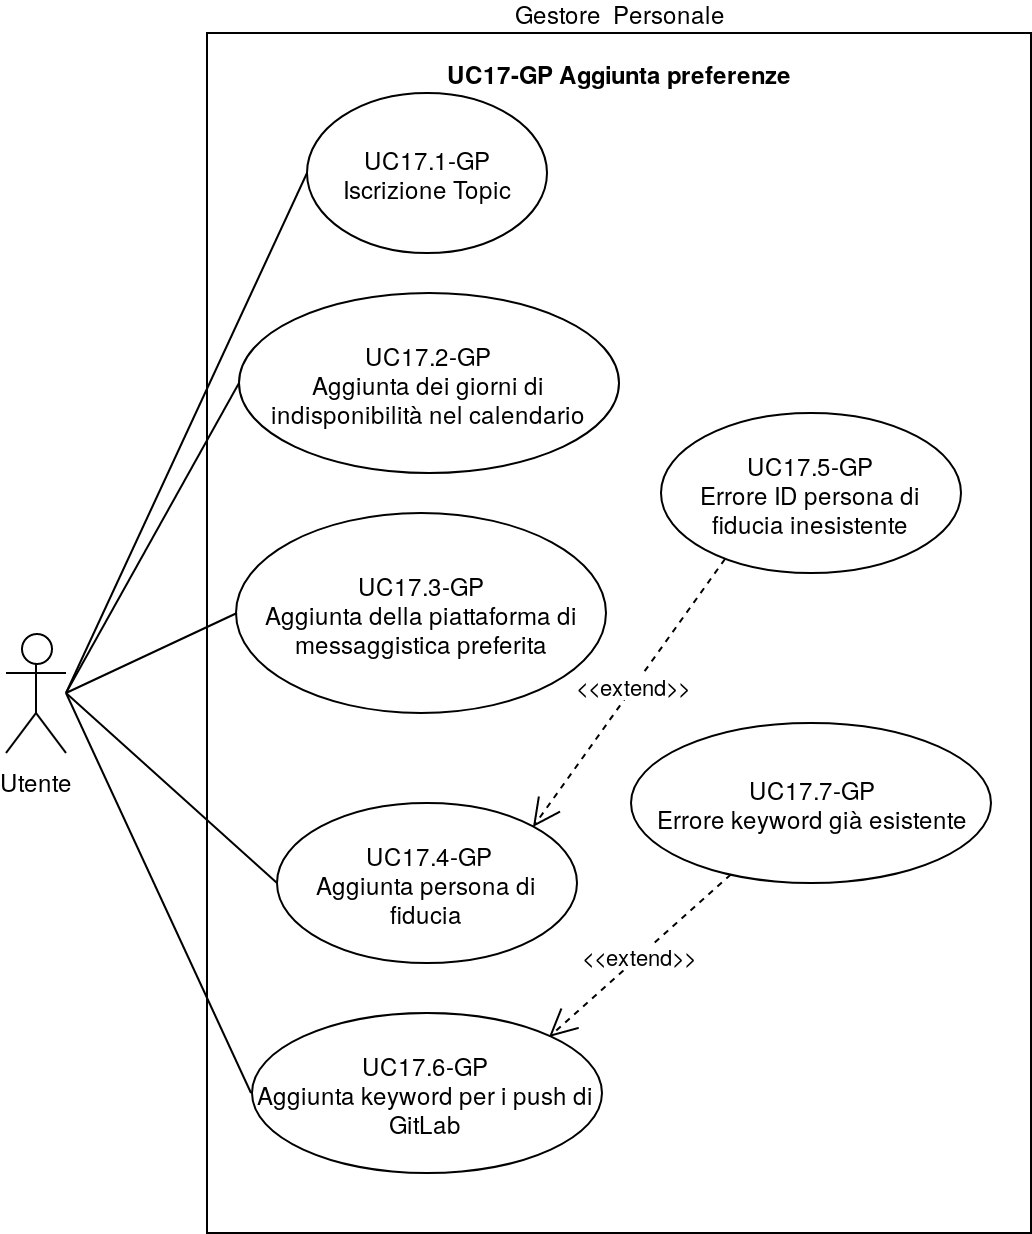
\includegraphics[width=1\textwidth]{img/casi_d'uso/UC17.png}\\
			\caption{UC\theuccount-GP - Aggiunta preferenze}
		\end{figure}
	\begin{itemize}
		\item \textbf{Codice}: UC\theuccount-GP.
		\item \textbf{Titolo}: aggiunta preferenze.
		\item \textbf{Attori primari}: utente.
		\item \textbf{Descrizione}: l’utente, date le varie opzioni per configurare Butterfly, aggiunge una
		preferenza tra Topic, giorni di calendario e la piattaforma di messaggistica (Telegram o Email) preferita
		\item \textbf{Precondizione}: l’utente ha acceduto con le sue credenziali corrette nel sistema e non ha già selezionato tutte le preferenze possibili proposte da \progetto.
		\item \textbf{Postcondizione}: la nuova configurazione contiene una o più preferenze in aggiunta rispetto a quella precedente.
		\item \textbf{Scenario principale}:
		\begin{enumerate}
			\item L'utente aggiunge una o più preferenze
		\end{enumerate}
	\end{itemize}

	\stepcounter{subuccount}
	\subsubsection{UC\theuccount.\thesubuccount-GP - Iscrizione Topic}

		\begin{itemize}
			\item \textbf{Codice}: UC\theuccount.\thesubuccount-GP.
			\item \textbf{Titolo}: iscrizione Topic.
			\item \textbf{Attori primari}: utente.
			\item \textbf{Descrizione}: data la lista di Topic presenti, l’utente ne seleziona uno o	più a cui è interessato, ricevendone una notifica. I Topic sono divisi per categoria e	comprendono etichette, progetto a cui sono legate e l'applicazione di provenienza: Redmine o GitLab.
			\item \textbf{Precondizione}: l’utente ha acceduto correttamente nel sistema e non ha già selezionato tutti i Topic possibili proposti da \progetto.
			\item \textbf{Postcondizione}: il numero di Topic a cui è interessato l’utente è aumentato.
			\item \textbf{Scenario principale}:
			\begin{enumerate}
				\item L'utente procede all'iscrizione di uno o più Topic
			\end{enumerate}
		\end{itemize}

	\stepcounter{subuccount}
	\subsubsection{UC\theuccount.\thesubuccount-GP - Aggiunta dei giorni di indisponibilità nel calendario}

		\begin{itemize}
			\item \textbf{Codice}: UC\theuccount.\thesubuccount-GP.
			\item \textbf{Titolo}: aggiunta dei giorni di indisponibilità nel calendario.
			\item \textbf{Attori primari}: utente.
			\item \textbf{Descrizione}: dato il calendario lavorativo, l’utente aggiunge uno o più giorni in cui non è reperibile e non vuole ricevere notifiche.
			\item \textbf{Precondizione}: l’utente ha acceduto correttamente nel sistema e vuole selezionare alcuni giorni di indisponibilità.
			\item \textbf{Postcondizione}: il numero di giorni in cui l’utente non si rende disponibile è aumentato.
			\item \textbf{Scenario principale}:
			\begin{enumerate}
				\item L'utente procede all'inserimento di uno o più giorni di indisponibilità
			\end{enumerate}
		\end{itemize}

	\stepcounter{subuccount}
	\subsubsection{UC\theuccount.\thesubuccount-GP - Aggiunta della piattaforma di messaggistica preferita}

		\begin{itemize}
			\item \textbf{Codice}: UC\theuccount.\thesubuccount-GP.
			\item \textbf{Titolo}: aggiunta della piattaforma di messaggistica preferita.
			\item \textbf{Attori primari}: utente.
			\item \textbf{Descrizione}: l’utente aggiunge la sua preferenza tra Telegram e Email dove vuole ricevere le notifiche.
			\item \textbf{Precondizione}: l’utente ha acceduto correttamente nel sistema e non ha già selezionato tutte le piattaforme di messaggistica possibili proposte da \progetto.
			\item \textbf{Postcondizione}: il numero di piattaforme di messaggistica selezionate dall’utente è aumentato.
			\item \textbf{Scenario principale}:
			\begin{enumerate}
				\item L'utente procede all'aggiunta di una o più piattaforme di messaggistica
			\end{enumerate}
		\end{itemize}

	% \stepcounter{subuccount}
	% \subsubsection{UC\theuccount.\thesubuccount-GP - Aggiunta persona di fiducia}

	% 	\begin{itemize}
	% 		\item \textbf{Codice}: UC\theuccount.\thesubuccount-GP.
	% 		\item \textbf{Titolo}: aggiunta persona di fiducia.
	% 		\item \textbf{Attori primari}: utente.
	% 		\item \textbf{Descrizione}: l’utente aggiunge l'utente legato a un identificativo di sua preferenza a cui inoltrare i messaggi in caso di indisponibilità.
	% 		\item \textbf{Precondizione}: l’utente ha acceduto con le sue credenziali corrette nel sistema e non ha già selezionato la persona a cui inoltrare le notifiche.
	% 		\item \textbf{Postcondizione}: la preferenza viene aggiunta correttamente.
	% 		\item \textbf{Scenario principale}:
	% 		\begin{enumerate}
	% 			\item L'utente procede all'aggiunta della sua persona di fiducia
	% 		\end{enumerate}
	% 		\item \textbf{Estensioni}:
	% 		\begin{enumerate}
	% 			\item Errore identificativo persona di fiducia inesistente [UC\theuccount.5-GP]
	% 		\end{enumerate}
	% 	\end{itemize}

	% \stepcounter{subuccount}
	% \subsubsection{UC\theuccount.\thesubuccount-GP - Errore identificativo persona di fiducia inesistente}

	% 	\begin{itemize}
	% 		\item \textbf{Codice}: UC\theuccount.\thesubuccount-GP.
	% 		\item \textbf{Titolo}: errore identificativo persona di fiducia inesistente.
	% 		\item \textbf{Attori primari}: utente.
	% 		\item \textbf{Descrizione}: l’utente cerca di aggiungere una persona di fiducia ma viene avvisato che ha inserito un identificativo errato.
	% 		\item \textbf{Precondizione}: l’utente ha acceduto con le sue credenziali corrette nel sistema e non ha già selezionato la persona a cui inoltrare le notifiche.
	% 		\item \textbf{Postcondizione}: il sistema comunica all’utilizzatore l’errore di preferenza.
	% 		\item \textbf{Scenario principale}:
	% 		\begin{enumerate}
	% 			\item L'utente procede all'aggiunta della sua persona di fiducia
	% 			\item Il sistema rileva che la persona di fiducia non esiste
	% 			\item L'utente visualizza l'errore
	% 		\end{enumerate}
	% 	\end{itemize}

	\stepcounter{subuccount}
	\subsubsection{UC\theuccount.\thesubuccount-GP - Aggiunta keyword per i push di GitLab}

		\begin{itemize}
			\item \textbf{Codice}: UC\theuccount.\thesubuccount-GP.
			\item \textbf{Titolo}: aggiunta keyword per i push di GitLab.
			\item \textbf{Attori primari}: utente.
			\item \textbf{Descrizione}: l’utente aggiunge le keyword che vuole che siano contenute nei messaggi di commit dei push di cui vuole ricevere la notifica.
			\item \textbf{Precondizione}: l’utente ha acceduto al sistema.
			\item \textbf{Postcondizione}: nelle nuove configurazioni dell'utente selezionato sono presenti una o più nuove keyword per ricevere le notifiche da push di GitLab di interesse.
			\item \textbf{Scenario principale}:
			\begin{enumerate}
				\item L'utente procede all'aggiunta di una o più nuove keyword
			\end{enumerate}
			\item \textbf{Estensioni}:
			\begin{enumerate}
				\item Errore keyword già esistente [UC\theuccount.7-GP]
			\end{enumerate}
		\end{itemize}

	\stepcounter{subuccount}
	\subsubsection{UC\theuccount.\thesubuccount-GP - Errore keyword già esistente}

	\begin{itemize}
		\item \textbf{Codice}: UC\theuccount.\thesubuccount-GP.
		\item \textbf{Titolo}: errore keyword già esistente.
		\item \textbf{Attori primari}: utente.
		\item \textbf{Descrizione}: la keyword che vuole aggiungere l'utente è già registrata nel sistema.
		\item \textbf{Precondizione}:  l’utente ha acceduto al sistema.
		\item \textbf{Postcondizione}: il sistema comunica all’utilizzatore l’errore della keyword.
		\item \textbf{Scenario principale}:
		\begin{enumerate}
			\item L'utente procede all'aggiunta di keyword
			\item Il sistema rileva che queste sono già presenti
			\item L'utente visualizza un messaggio di errore
		\end{enumerate}
	\end{itemize}